\documentclass[10pt, compress, aspectratio=169]{beamer}

% Professional Executive Palette (Muted Deep Slate Navy & Steel Accent - Non-Radiant)
\definecolor{BTPPrimary}{RGB}{20, 50, 80}     % Deep Slate Navy (Muted, professional)
\definecolor{BTPSecondary}{RGB}{45, 100, 140} % Steel Slate Blue Accent
\definecolor{BTPGreen}{RGB}{46, 125, 50}      % Muted Forest Green
\definecolor{BTPRed}{RGB}{180, 40, 40}        % Muted Crimson Red
\definecolor{BTPBg}{RGB}{246, 248, 250}       % Soft Light Canvas

% Modern Metropolis Theme Setup
\usetheme[progressbar=frametitle, numbering=none]{metropolis}
\setbeamertemplate{frame numbering}[none]
\setbeamercolor{background canvas}{bg=white}
\setbeamercolor{normal text}{fg=black}
\setbeamercolor{frametitle}{bg=white, fg=BTPPrimary}
\setbeamercolor{progress bar}{fg=BTPSecondary, bg=gray!20}
\setbeamercolor{block title}{bg=BTPPrimary, fg=white}
\setbeamercolor{block body}{bg=BTPBg, fg=black}
\setbeamercolor{section title}{fg=BTPPrimary}

\setbeamertemplate{frame footer}{DyMATES — Dynamic Traffic Enforcement System}
\setbeamertemplate{navigation symbols}{}

\usepackage{appendixnumberbeamer}
\usepackage{booktabs}
\usepackage{tabularx}
\usepackage{hyperref}
\usepackage{colortbl}
\usepackage{tikz}
\usepackage{pgfplots}
\pgfplotsset{compat=1.18}
\usetikzlibrary{shapes.geometric, arrows, positioning}

\title{DyMATES}
\subtitle{Dynamic Multi-Agent Traffic Enforcement System}
\date{September 15, 2026}
\author{DyMATES Core Development Team}
\institute{Department of Computer Science \& Engineering}

\begin{document}

% =========================================================================
% SLIDE 1: Title Slide
% =========================================================================
\maketitle

% =========================================================================
% SLIDE 2: Project Overview & Architecture Diagram
% =========================================================================
\begin{frame}{Project Overview \& 5-Layer System Architecture}
    \begin{columns}[T]
        \column{0.48\textwidth}
        \textbf{\textcolor{BTPPrimary}{Unified 4-in-1 Enforcement Concept}}
        \vspace{2mm}
        
        Real-time AI enforcement from standard CCTV feeds:
        \vspace{2mm}
        
        \begin{itemize}\small
            \item \textbf{\textcolor{BTPRed}{No-Helmet Detection}} -- Helmet compliance check.
            \item \textbf{\textcolor{BTPRed}{Triple Riding Offenses}} -- Multi-occupant load counting.
            \item \textbf{\textcolor{BTPRed}{Wrong-Way Driving}} -- Direction flow tracking.
            \item \textbf{\textcolor{BTPRed}{Rash / Reckless Driving}} -- Trajectory swerving analysis.
        \end{itemize}
        \vspace{2mm}
        Replaces multi-camera setups with a single smart AI pipeline.

        \column{0.52\textwidth}
        \textbf{\textcolor{BTPPrimary}{5-Layer Workflow Pipeline}}
        \vspace{2mm}
        \begin{center}
            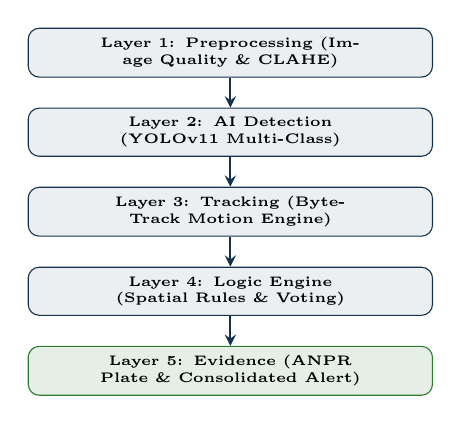
\begin{tikzpicture}[
                node distance=0.38cm, 
                box/.style={rectangle, draw=BTPPrimary, rounded corners=4pt, fill=BTPPrimary!8, text=black, text centered, text width=4.9cm, minimum height=0.50cm, font=\tiny\bfseries},
                arrow/.style={thick,->,draw=BTPPrimary,>=stealth}
            ]
                \node (l1) [box] {Layer 1: Preprocessing (Image Quality \& CLAHE)};
                \node (l2) [box, below=of l1] {Layer 2: AI Detection (YOLOv11 Multi-Class)};
                \node (l3) [box, below=of l2] {Layer 3: Tracking (ByteTrack Motion Engine)};
                \node (l4) [box, below=of l3] {Layer 4: Logic Engine (Spatial Rules \& Voting)};
                \node (l5) [box, below=of l4, fill=BTPGreen!12, draw=BTPGreen] {Layer 5: Evidence (ANPR Plate \& Consolidated Alert)};

                \draw [arrow] (l1) -- (l2);
                \draw [arrow] (l2) -- (l3);
                \draw [arrow] (l3) -- (l4);
                \draw [arrow] (l4) -- (l5);
            \end{tikzpicture}
        \end{center}
    \end{columns}
\end{frame}

% =========================================================================
% SLIDE 3: Dataset Description & Implementation Details
% =========================================================================
\begin{frame}{Dataset Specifications \& Implementation Stack}
    \begin{columns}[c]
        \column{0.50\textwidth}
        \metroset{block=fill}
        \begin{block}{Dataset Specifications}
            \begin{itemize}\scriptsize
                \item \textbf{Dataset URL}: \href{https://huggingface.co/datasets/keremberke/helmet-detection}{\textcolor{BTPSecondary}{\underline{keremberke/helmet-detection}}}
                \item \textbf{Total Annotated Images}: \textbf{5,693 Images}
                \item \textbf{Data Split}: 5,061 Train / 632 Val / 634 Test
                \item \textbf{Target Classes}:
                \begin{itemize}\tiny
                    \item \textsf{with\_helmet} (3,391 instances)
                    \item \textsf{without\_helmet} (2,306 instances)
                    \item \textsf{motorcycle} (Vehicle spatial linking)
                    \item \textsf{license\_plate} (Dual-crop ANPR)
                \end{itemize}
            \end{itemize}
        \end{block}

        \column{0.50\textwidth}
        \metroset{block=fill}
        \begin{block}{Implementation Technology Stack}
            \begin{itemize}\small
                \item \textbf{Core AI Engines}: YOLOv11 + ByteTrack + PaddleOCR v2.7.
                \item \textbf{Framework}: PyTorch 2.11 / OpenCV / Streamlit / SQLite3.
                \item \textbf{Deployment}: \textsf{/home/chidwipak/Jeevan/BTP/DyMATES} (Live Dashboard running on Port 8501 / 8502).
            \end{itemize}
        \end{block}
    \end{columns}
\end{frame}

% =========================================================================
% SLIDE 4: Key Advancement 1 - High-Precision Detection Model
% =========================================================================
\begin{frame}{Key Advancement 1: High-Precision AI Detection Model}
    \begin{columns}[c]
        \column{0.50\textwidth}
        \textbf{\textcolor{BTPPrimary}{Model Fine-Tuning \& Gains}}
        \vspace{2mm}
        \begin{itemize}\small
            \item Fine-tuned single-pass YOLOv11 model trained on 5,693 traffic dataset images.
            \item Simultaneously detects motorcycles, helmets, unhelmeted heads, and license plates in real time.
        \end{itemize}
        
        \vspace{3mm}
        \begin{itemize}\small
            \item \textbf{Overall Accuracy}: \textbf{\textcolor{BTPGreen}{90.4\% mAP@50}} (\textbf{+32.9\% Gain}).
            \item \textbf{Detection Precision}: \textbf{90.0\% Precision}.
            \item \textbf{No-Helmet Alert Accuracy}: \textbf{90.5\% mAP@50}.
        \end{itemize}

        \column{0.50\textwidth}
        \begin{block}{Accuracy Growth Chart}
            \begin{center}
                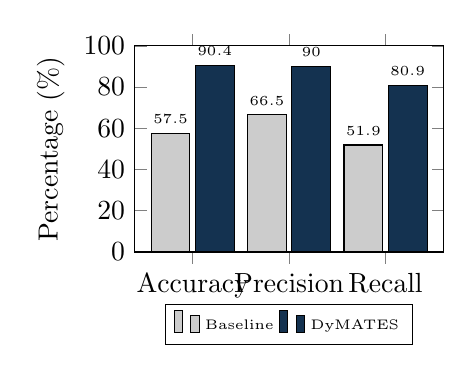
\begin{tikzpicture}
                    \begin{axis}[
                        ybar,
                        height=4.2cm, width=5.5cm,
                        bar width=14pt,
                        symbolic x coords={Accuracy, Precision, Recall},
                        xtick=data,
                        nodes near coords,
                        nodes near coords align={vertical},
                        nodes near coords style={font=\tiny\bfseries},
                        ylabel={Percentage (\%)},
                        ymin=0, ymax=100,
                        legend style={at={(0.5,-0.25)}, anchor=north, legend columns=-1, font=\tiny},
                        enlarge x limits=0.3,
                    ]
                    \addplot[fill=gray!40, draw=black] coordinates {(Accuracy, 57.5) (Precision, 66.5) (Recall, 51.9)};
                    \addplot[fill=BTPPrimary, draw=black] coordinates {(Accuracy, 90.4) (Precision, 90.0) (Recall, 80.9)};
                    \legend{Baseline, DyMATES}
                    \end{axis}
                \end{tikzpicture}
            \end{center}
        \end{block}
    \end{columns}
\end{frame}

% =========================================================================
% SLIDE 5: Key Advancement 2 - Multi-Rider & Triple Riding Detection
% =========================================================================
\begin{frame}{Key Advancement 2: Multi-Rider \& Triple Riding Detection}
    \begin{columns}[c]
        \column{0.50\textwidth}
        \textbf{\textcolor{BTPPrimary}{Smart Passenger Load Counting}}
        \vspace{2mm}
        \begin{itemize}\small
            \item Counts all riders on a motorcycle, whether wearing helmets or not, to accurately detect triple riding.
            \item Widens the detection area around motorcycles to reliably capture rear seat passengers.
            \item Groups nearby riders together even if the motorcycle body is partially occluded.
        \end{itemize}

        \column{0.50\textwidth}
        \metroset{block=fill}
        \begin{block}{Key Operational Benefits}
            \begin{itemize}\small
                \item Prevents missed offenses when riders wear helmets.
                \item Reliably flags 3 or more occupants on any two-wheeler.
                \item Ensures sidewalk pedestrians are never misflagged for traffic violations.
            \end{itemize}
        \end{block}
    \end{columns}
\end{frame}

% =========================================================================
% SLIDE 6: Key Advancement 3 - Smooth Video Motion & Auto Direction Learning
% =========================================================================
\begin{frame}{Key Advancement 3: Smooth Video Motion \& Auto Direction Learning}
    \begin{columns}[c]
        \column{0.50\textwidth}
        \textbf{\textcolor{BTPPrimary}{Smooth Motion Tracking}}
        \vspace{2mm}
        \begin{itemize}\small
            \item Smooths out camera bounding box movement so normal vehicles are not wrongly flagged for rash driving.
            \item Accurately detects real erratic swerving and reckless driving behavior.
            \item Maintains vehicle tracking IDs even when bikes pass behind buses or large vehicles.
        \end{itemize}

        \column{0.50\textwidth}
        \metroset{block=fill}
        \begin{block}{Adaptive Traffic Direction}
            \begin{itemize}\small
                \item Automatically learns normal traffic flow direction on any road or junction.
                \item Detects wrong-way driving on curved roads, angled camera poles, or complex intersections.
                \item Requires zero manual setup or angle configuration.
            \end{itemize}
        \end{block}
    \end{columns}
\end{frame}

% =========================================================================
% SLIDE 7: Key Advancement 4 - License Plate Reading & Multi-Frame Voting
% =========================================================================
\begin{frame}{Key Advancement 4: License Plate Reading \& Multi-Frame Voting}
    \begin{columns}[c]
        \column{0.50\textwidth}
        \textbf{\textcolor{BTPPrimary}{Image Quality Enhancement}}
        \vspace{2mm}
        \begin{itemize}\small
            \item Enhances license plate image contrast and removes dark shadows for clear reading.
            \item Validates extracted plate numbers against standard Indian license plate patterns.
            \item Sharpens blurred character edges to improve OCR accuracy.
        \end{itemize}

        \column{0.50\textwidth}
        \metroset{block=fill}
        \begin{block}{Multi-Frame Majority Voting}
            \begin{itemize}\small
                \item Reads the license plate across 5--10 consecutive video frames for each moving vehicle.
                \item Picks the most frequent character sequence through majority consensus.
                \item Eliminates single-frame motion blur and character misreads (e.g., \textbf{O} vs \textbf{0}).
            \end{itemize}
        \end{block}
    \end{columns}
\end{frame}

% =========================================================================
% SLIDE 8: Key Advancement 5 - Anti-Spam Guard & Single Consolidated Emails
% =========================================================================
\begin{frame}{Key Advancement 5: Anti-Spam Guard \& Single Consolidated Emails}
    \begin{columns}[c]
        \column{0.50\textwidth}
        \textbf{\textcolor{BTPPrimary}{Anti-Spam Ticket Guard}}
        \vspace{2mm}
        \begin{itemize}\small
            \item Uses a 5-second per-vehicle cooldown buffer to prevent duplicate ticket generation.
            \item Issues \textbf{exactly 1 clean ticket per incident} into the database.
            \item Provides 1-click CSV export for official traffic enforcement records.
        \end{itemize}

        \column{0.50\textwidth}
        \metroset{block=fill}
        \begin{block}{Consolidated Image Email Alerts}
            \begin{itemize}\small
                \item Uploading an image with multiple infractions dispatches \textbf{ONE SINGLE CONSOLIDATED EMAIL}.
                \item Summarizes all identified offenses in clear cards with 4K HD proof images attached inline.
                \item Prevents email inbox spamming by combining offenses into a single official report.
            \end{itemize}
        \end{block}
    \end{columns}
\end{frame}

% =========================================================================
% SLIDE 9: E-Challan Output - Sample Alert Ticket Structure
% =========================================================================
\begin{frame}{E-Challan Email Output: Sample Alert Ticket Structure}
    \begin{columns}[c]
        \column{0.48\textwidth}
        \textbf{\textcolor{BTPPrimary}{Email Alert Features}}
        \vspace{2mm}
        \begin{itemize}\small
            \item \textbf{Subject Header}: \textsf{🚨 CONSOLIDATED E-CHALLAN ALERT [CH-IMG-15090312]: 2 Infraction(s) [NO\_HELMET, TRIPLE\_RIDING]}
            \item \textbf{Standalone Unthreading}: Custom headers guarantee individual alert delivery directly in Gmail.
            \item \textbf{Inline Evidence}: High-resolution proof images with clear red violation boxes embedded inside the email.
        \end{itemize}

        \column{0.52\textwidth}
        \metroset{block=fill}
        \begin{block}{Sample Consolidated Ticket Structure}
            \begin{center}\small
                \begin{tabularx}{\textwidth}{lX}
                    \rowcolor{BTPPrimary!15}
                    \textbf{Field} & \textbf{Consolidated E-Challan Value} \\
                    \hline
                    \textbf{Report Code} & \textsf{CH-IMG-15090312-A1B2C3D4} \\
                    \textbf{Timestamp} & \textsf{2026-09-15 03:24:14 IST} \\
                    \textbf{Primary Plate} & \textsf{TS09AB1234} (ANPR OCR) \\
                    \textbf{Offense \#1} & \textcolor{BTPRed}{\textbf{NO\_HELMET}} (Conf: 89.0\%) $\rightarrow$ Proof 1 \\
                    \textbf{Offense \#2} & \textcolor{BTPRed}{\textbf{TRIPLE\_RIDING}} (Conf: 94.0\%) $\rightarrow$ Proof 2 \\
                    \textbf{Recipient} & \textsf{jeevankumarkotati@gmail.com} \\
                \end{tabularx}
            \end{center}
        \end{block}
    \end{columns}
\end{frame}

% =========================================================================
% SLIDE 10: Master Performance & Capability Comparison
% =========================================================================
\begin{frame}{Master Performance \& Capability Comparison}
    \begin{center}
        \small
        \renewcommand{\arraystretch}{1.42}
        \begin{tabularx}{0.98\textwidth}{lXX}
            \rowcolor{BTPPrimary!15}
            \textbf{Core System Area} & \textbf{Initial Baseline System} & \textbf{Enhanced DyMATES Pipeline} \\
            \hline
            \rowcolor{BTPBg}
            \textbf{Detection Accuracy} & 57.5\% mAP@50 (Frequent misses) & \textbf{\textcolor{BTPGreen}{90.4\% mAP@50 (+32.9\% Accuracy Gain)}} \\
            \textbf{Triple Riding Check} & Excluded helmeted riders & \textbf{\textcolor{BTPGreen}{Inclusive Occupant Counting + Spatial Cluster}} \\
            \rowcolor{BTPBg}
            \textbf{Vehicle Motion Analysis} & Box jitter false rash flags & \textbf{\textcolor{BTPGreen}{Trajectory Motion Smoothing (0 False Flags)}} \\
            \textbf{License Plate OCR} & Blurry single-frame cutouts & \textbf{\textcolor{BTPGreen}{2$\times$ CLAHE + Multi-Frame Majority Voting}} \\
            \rowcolor{BTPBg}
            \textbf{E-Challan Dispatch} & Multiple email spam per image & \textbf{\textcolor{BTPGreen}{1 Consolidated Email per Image + HD Proof}} \\
            \textbf{Database Archival} & Duplicate spam entries & \textbf{\textcolor{BTPGreen}{Anti-Spam Cooldown Guard + CSV Export}} \\
            \hline
        \end{tabularx}
    \end{center}

    \vspace{2.5mm}
    \begin{center}
        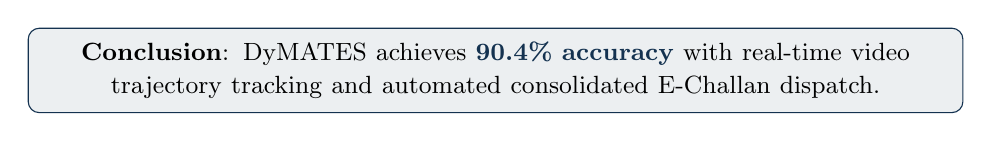
\begin{tikzpicture}
            \node[fill=BTPPrimary!8, draw=BTPPrimary, rounded corners=4pt, inner sep=5pt, text width=0.95\textwidth, align=center] {
                \small \textbf{Conclusion}: DyMATES achieves \textbf{\textcolor{BTPPrimary}{90.4\% accuracy}} with real-time video trajectory tracking and automated consolidated E-Challan dispatch.
            };
        \end{tikzpicture}
    \end{center}
\end{frame}

\end{document}
